\subsection{Z-Axis: Horizontal Data Partitioning}
\label{sec:z-axis}

The direction taken by scaling on the y-axis is to segment based on the service,
i.e. based on \emph{dissimilar} things. Scaling on the z-axis means segment on
\emph{similar} things, thus making the segmentation biased by the data or the
actions that are unique to the sender or the receiver of the request. In
particular, to enhance significantly the system a z-axis split should partition
both transactions and the data necessary to perform the transactions. An example
of such scaling could be, in a client-server architecture, the geographic
distribution of the servers based on the clients requests, such that a request
performed in Europe is undertaken by a server located in Europe instead of one
located on the other side of the globe. One similar example of successful z-axis
split is sharding.

\subsubsection{An example: Sharding}
Sharding is commonly used in distributed databases to scale \emph{horizontally}
by splitting the data of a single database in several servers. This way, it is
possible to augment the transaction throughput by adding more machines, instead
of requiring a more powerful machine, as in the case of \emph{vertical} scaling.
%The idea of horizontal scaling comes in handy when the database is hosted in
%the cloud, where usually the available machines have a limited power.
Indeed, when the number of requests grows, the resources of a single server
could be insufficient to grant acceptable response times. The drawback of using
multiple servers is the management overhead.

\begin{figure}
  \begin{center}
    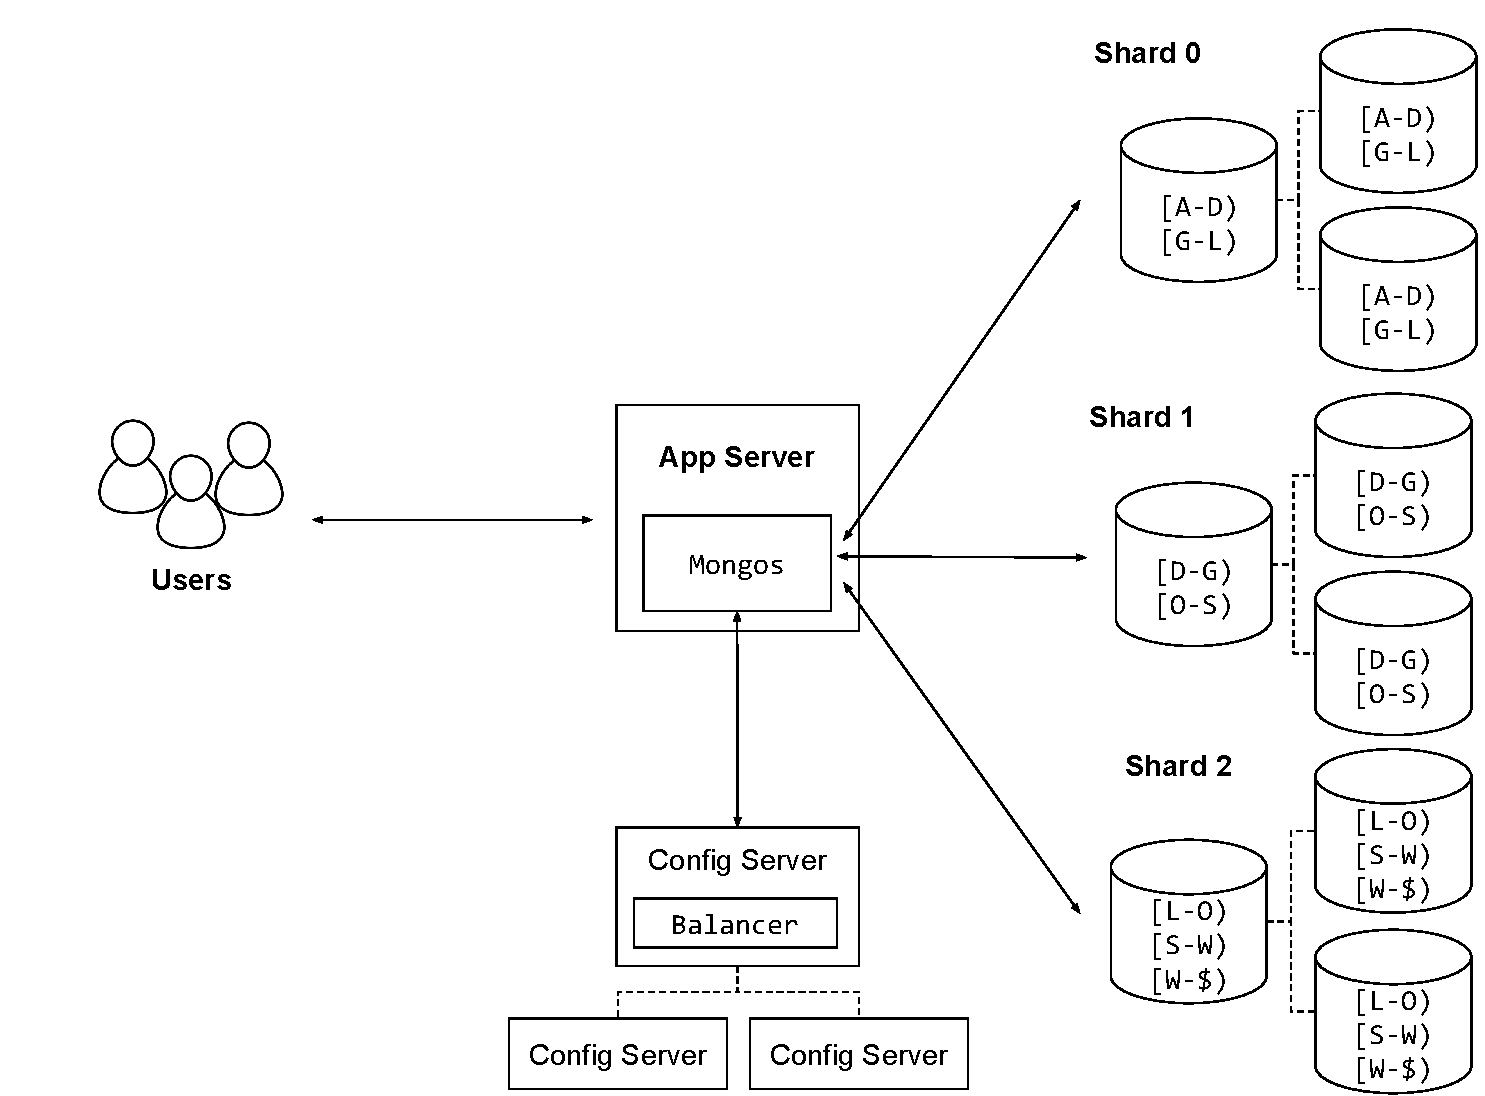
\includegraphics[width=0.7\textwidth]{./res/img/mongodb}
    \caption{A typical architecture of an application server with a sharded
    MongoDB database.}
    \label{fig:mongodb}
  \end{center}
\end{figure}

One emblematic example of implementation of (auto-)sharding is
MongoDB\footnote{\url{https://www.mongodb.com/}}~\cite{bib:mongodb}. This kind
of open-source NoSQL database stores documents without a fixed schema.
%In addition to auto-sharding, MongoDB has several compelling features, such as
%replication, aggregation framework and map-reduce. We will describe only
%sharding because the other features are beyond the scope of this report. We
%will refer to~\cite{} for a description of the other key features of MongoDB.
MongoDB gives the possibility to split a collection of documents into different
\emph{shards} according to a selected \emph{shard key} and a \emph{sharding
strategy}. Each shard consists of one or more replicated servers\footnote{In
MongoDB jargon it is known as \emph{replica set}.} and it is accountable to
store the documents in a partition of the key space. These partitions are
composed of one or more chunks. These are minimal piece of data (default 64MB)
that contain the documents, whose shard key values are included within a
contiguous range of the key space. To have a unique correspondence between
documents and chunk, and transitively of documents and shard, no overlapping
chunks are permitted. If after inserting new documents in a given chunk, it
exceeds a configured size, the chunk is split. Furthermore, if a shard contains
too many chunks, some of them may be migrated to other shards.

Since the users and the applications should be able to access the data
\emph{transparently}, that is without knowing where the documents are really
stored, an entity called \texttt{mongos} is introduced. Essentially, it is a
broker between the application and the database, that forwards the requests to
the right shard(s), collects the responses and returns them to the requester.
Usually each application has its own \texttt{mongos} instance, but other
configurations are also possible~\cite{bib:mongodb}.

%Mongos should know where to search the documents according to the shard key,
%therefore MongoDB maintain an up-to-date table that associate uniquely a chunk
%with a shard.
In order to know where the data are stored, the \texttt{config servers} are
used. They contain metadata and the configuration settings for the cluster, such
as the list of chunks that are stored in each shard and the ranges covered by
the chunks. Each time a chunk is split or migrated these settings should be
updated.
%Since all replicas should have the same information about the list of chunks
%and their actual location, chunks can be split and migrated only if all
%\texttt{config servers} are up and running.

To automatically balance the load between the different shards, a background
process in the principal \texttt{config server} called \emph{sharded cluster
balancer} is employed\footnote{In version prior to 3.4 (the current version is
4.0) the role balancer was played by the different \texttt{mongos} instances on
turn~\cite{bib:mongodb-docs}}. It monitors constantly the number of chunks on
each shard and  whenever one  shard contains more chunks than a given threshold,
it tries to migrate chunks to balance the amount of chunks in each shards. In
addition, it attempts to minimize the amount of data that should be migrated to
reduce the performance impact due to the bandwidth and workload consumption
caused by migration. For example, one shard cannot be involved in more than one
migration at the same time. Moreover, if additional servers are available, the
balancer may also create new shards or it may simply rearrange the partitions.

These concepts are summarized in~\autoref{fig:mongodb}, in which the replicas
are bounded with dashed lines whereas the solid lines represents which component
communicates with which one. The chunks are shown with the ranges of the shard
key space they cover. Whenever the application server must query the database to
collect information, it demands the mongos instance to do so. If the query
contains the shard-key, the broker can forward the request to the right
shard(s). When this information is not available, \texttt{mongos} should
broadcast the request to all the shards.

% EXAMPLE
We clarify this by means of an example. Let's take into
consideration~\autoref{fig:mongodb} and suppose that the sharded database
contains the collections of users of the system of the application server, which
needs the data related to a user to perform authentication. Furthermore, suppose
that the shard key is the username and that the chunks are split according to
the initial letter of the username. Now, if the application server needs the
data belonging to a certain user, let's say \texttt{JohnDoe}, it has to create a
query and send it to the \texttt{mongos} instance. This searches in the
\texttt{config server} which chunk \emph{should contain} the searched key and
discover that shard-0 contains the chunk ranging from G to L and therefore
forwards the request to shard-0 and obtains the awaited response.
\texttt{mongos} elaborates it and send the reply to the application server, that
can now use the information. However, if the query does not contain the shard
key, the broker has no way to know in which shard the information is stored and
has to broadcast the request. It is worth to notice that the choice of the shard
key is fundamental to grant a certain level of performance. If the server is
sharded according to, let's say, the age of the users, the search by username
would require a broadcast, because in the \texttt{config server} there would be
no information to forward the request to the shard containing the required
document.


\subsubsection{Ethereum current state and proposals}
We argue that currently Ethereum is not developed in the z-axis, because each
node of the network should have information about the whole blockchain and the
status of all accounts in the network (\autoref{sec:world-state}) to process the
transactions. For this reason Ethereum cannot be more efficient than a single
machine, as already pointed out by Vitalik Buterin in the muave
paper~\cite{bib:mauve}.

Furthermore, a z-axis split similar in nature with the one of MongoDB, i.e. by
letting different nodes store different part of the state would surely diminish
the amount of data to store on each node, but
\begin{enumerate*}[label=(\Alph*)]
  \item it would require a lot of data to be sent across the network to perform
  the computations, and
  \item it would not augment the transaction throughput, but rather diminish it.
  %    \item finally, it would betray one of the fundamental principles of the
  %    permissionless blockchains, namely the trust to other parties.
\end{enumerate*}
To justify point (A) we consider that many computations require the ability to
access a fair amount of addresses and their storage as the following example
clarifies. Let's consider the process of a transaction that requires some
computations on the EVM. To complete this action we need several information,
such as the balance of the sender of the transaction and the code of the
contract invoked. In turn, the contract invoked may call other contracts and so
on. In addition, these may modify the balance of other accounts as a side
effect, e.g. through the \texttt{SELFDESTRUCT}\footnote{This opcode causes the
deletion of the executing contract from the world state and sends the balance of
the contract to a selected account~\cite{wood2018ethereum}.} opcode. Thus, to
process a transaction we need the account states of the sender and the called
contracts and all account state that are affected by the computations. The point
(A) implies points (B), indeed the overhead due to the communication would
surely slow down the transaction processing action.

With these considerations in mind and by recalling that to be significant a
z-axis split should partition both the transactions and the data necessary to
perform the transactions, more clever approaches were proposed.

To tackle a z-axis split, we can identify different proposals, among which
Plasma and Sharding. The Plasma proposal is categorized as an \emph{off-chain}
solution because it executes some transactions outside the main chain. At the
opposite, in which the sharding belongs, the \emph{on-chain} solutions execute
every transaction on the main chain. Typically, in order to apply an off-chain
solution, one or more smart contracts are sufficient (for example, Vitalik
proposed a specification for a minimal implementation called Minimum Viable
Plasma\footnote{\url{https://ethresear.ch/t/minimal-viable-plasma/426}}), while
an on-chain solution requires an hard-fork.

\subsubsection{Plasma}

\begin{figure}[t]
    \begin{center}
        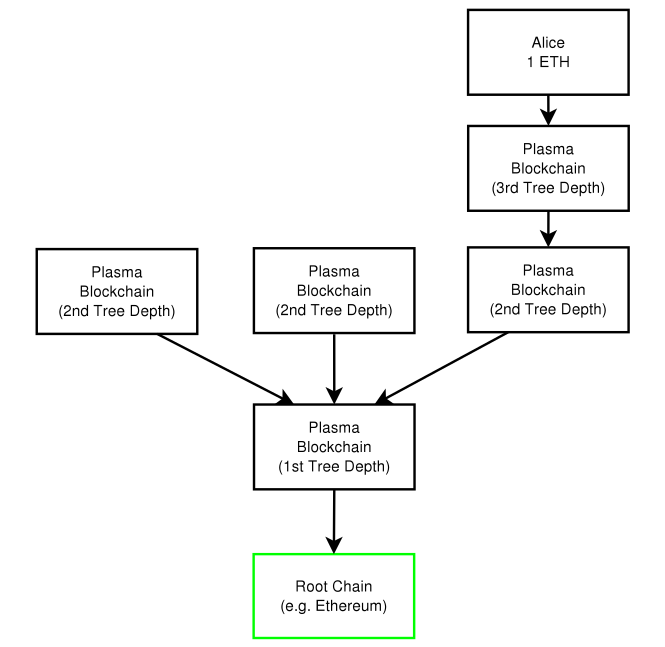
\includegraphics[width=0.7\textwidth]{./res/img/plasma}
        \captionsource{Plasma hierarchical tree structure
            representation.}{\url{https://plasma.io/plasma.pdf}}
        \label{fig:plasma}
    \end{center}
\end{figure}

The idea of Plasma is to create a tree hierarchy of blockchains. Each chain
refers to a parent chain, except the root (i.e. the main chain, Ethereum in our
case). Plasma consists of a series of smart contracts which allows for many
blockchains within a root blockchain~\cite{poon2017plasma} as represented
in~\autoref{fig:plasma}. The Plasma blockchains co-exist with their own business
logic and all the computations are enforced at root level only in the event of
proof of fraud, and only the block header hashes are submitted. During
non-faulty states, only merkleized commitments are periodically broadcast to the
root blockchain. The efficiency mainly comes from this last feature since
multiple state updates can be condensed in a single state update in the root
chain. This system design implies that most of the computation can be done
off-chain (i.e. outside the root chain) and the state is enforced on-chain (i.e.
in the root chain). Significant scalability for the users is achieved through
chain split: when a Plasma blockchain grows too large, it can be split in child
chains allowing the users to observe only Plasma blockchains in which their
funds resides.

\subsubsection{Sharding in Ethereum}
The Ethereum foundation~\cite{bib:mauve, bib:sharding-faq} and the scientific
community~\cite{bib:scaling-croman} have proposed sharding combined with
Proof-of-Stake (\emph{shasper}\footnote{This name is obtained by the contraction
of the words \emph{sharding} and \emph{Casper}, the Ethereum's Proof of Stake
proposal~\cite{bib:cbc-casper}.}) as an effective measure to dramatically
increase the transaction throughput. Although the details about this proposal
are constantly
updating\footnote{\url{https://notes.ethereum.org/SCIg8AH5SA-O4C1G1LYZHQ}} and
there is no reference implementation\footnote{The Prysmatic Labs company is
modifying the \texttt{geth} implementation to implement both PoS and sharding
(\url{https://github.com/prysmaticlabs/prysm}), but it is far from being
production ready.}, we will report here the basic
ideas~\cite{bib:mauve,bib:sharding-faq} about sharding and explain why this
approach could improve the scalability of the system.

The Ethereum sharding proposal consists in splitting the world state and
transaction history into different partitions called shards. Each shard is a
distinct universe, i.e. is itself a PoS chain, in which the transactions affect
only the accounts in the same shard. The transactions affecting one shard are
collected in so-called \emph{collations} by members of the network known as
\emph{proposers}. Collations are the analogous of blocks at the shard level and
like blocks (\autoref{fig:world-state}) are chained and contain several fields,
among which the list of transactions and the address of the proposer. Once per
\emph{epoch}, a block in the main PoS chain (main block) is created, where
\emph{cross-links} (e.g. the hash of the collations) to the accepted shard
collations are inserted. The collations are accepted or refused by a committee
of \emph{attesters}. To become an attester or a proposer the members of the
network should deposit an amount of ether. After this operation, they can be
randomly assigned to different shards. This is done in order to grant a certain
level of decentralization and security.

This sharding proposal allows to process the transactions of different shards in
parallel and therefore significantly increase the transaction throughput.
Another major benefit of this approach is that the nodes in one shard should
verify only the transactions in their shard rather than verifying all the
transactions.

This simplified description of sharding do not take into consideration the
communication between different shards, but obviously it is a desirable
characteristics. Thus, cross-sharding communication mechanisms were
proposed~\cite{bib:sharding-faq}.

Moreover, one important feature that is desirable and planned is the
transparency of sharding to smart contract developers~\cite{bib:sharding-faq}.
